\chapter{Tworzenie polskich zbiorów}
W ostatnim czasie w szczególności nacisk zostaje przenoszony z modeli na odpowiednie przygotowanie i jakość zbiorów danych. Przykładem tego jest wydany w ostatnim czasie artykuł \bibtitle{Textbooks are all you need} \cite{Gunasekar2023}, który demonstruję jak dużą poprawę można uzyskać bez powiększania i komplikowania wykorzystywanego modelu, lecz poprzez stworzenie wysokiej jakości zbioru danych.

Jako, że dla zadania \code{Text-to-SQL} na moment pisania niniejszej pracy nie istnieją żadne zbiory danych w języku polskim, a także ze względu na duże ich znaczenie, wiele uwagi zostało poświęcone tej kwestii. 

Na początku bieżącego rozdziału omówione zostaną przyjęte założenia dotyczące tworzenia polskich zbiorów, a następnie przedyskutowane dokładnie dwa kluczowe dla tego procesu elementy: dynamiczne generowanie oraz sposób dokonywania tłumaczenia. Ostatecznie nastąpi analiza i podsumowanie stworzonych zbiorów.

\section{Przyjęte założenia}
Po przeanalizowaniu różnic pomiędzy istniejącymi tłumaczeniami zbioru \code{Spider} określone zostały założenia przyjęte na potrzebę stworzenia zbiorów polskich.

% To fix:
Podczas tłumaczenia zbiorów przyjęto dwa podstawowe założenia. Pierwszym jest wykorzystanie tłumaczenia maszynowego, zamiast manualnego. Drugi stanowi dynamiczne generowanie finalnych zbiorów zamiast jednorazowego tłumaczenia wszystkich przykładów i udostępnienia jedynie zmodyfikowanej ich wersji. Oba założenia zostaną rozwinięte, uzasadnione i dokładnie przedyskutowane w poniższych dwóch sekcjach.

\subsubsection{Tłumaczenie maszynowe}
Pomimo wskazanej w sekcji \ref{text:translation-method} dominacji tłumaczenia manualnego nad maszynowym postanowiono wykorzystać to ostatnie. Przyczyn takiej decyzji jest kilka. Przede wszystkim w realizację tłumaczenia aktywnie zaangażowana jest jedynie jedna osoba, w odróżnieniu do wcześniejszych prac, w których w tym procesie uczestniczyło ich kilka, a w przypadku rosyjskiego zbioru nawet profesjonalny tłumacz. Drugą przesłanką jest ograniczony czas, ze względu na pracę magisterką w ramach której niniejszy temat jest realizowany. Ostatecznie jest to zadanie żmudne, a zbiór maszynowy, pomimo niższej jakości, także pozwoli, a nawet da więcej czasu, na wykonanie eksperymentów.

\subsubsection{Dynamiczne generowanie}
Wszystkie dotychczasowe tłumaczenia zbioru Spider sprowadzają się jedynie do udostępnienia zmodyfikowanej wersji zbioru, bez żadnych dodatkowych skryptów. Wydaje się to wystarczające i dla większości zastosowań w rzeczywistości jest. Taki zbiór stanowi bardzo dobry benchmark służący do porównywania różnych algorytmów, ponieważ nie ma żadnych niedomówień w kwestii jego zawartości.

Podjęcie innowacyjnego podejścia polegającego na generowaniu finalnego zbioru z odpowiednio przygotowanych elementów składowych ma jednak szereg zalet. Jedną z nich jest brak konieczności podejmowania kategorycznej decyzji odnośnie wyboru języka schematu baz danych - można wygenerować różne warianty podając różne parametry do polecenia generującego. Podobnie nie trzeba decydować, czy wartości w zapytaniach SQL mają być tłumaczone. Jest to więc podejście bardzo elastyczne i otwierające drogę do przeprowadzania różnorodnych eksperymentów.

\subsubsection{Oryginalna zawartość baz danych}
Zawartość baz danych postanowiono pozostawić bez tłumaczenia. Jest to podejście pokrywające się z większością istniejących tłumaczeń zbioru \code{Spider}. Powodem do tego jest duża ilość znajdujących się w bazach informacji, których tłumaczenie skutkowałoby naliczeniem dodatkowych kosztów. Oferowane przez użyty tłumacz DeepL darmowe limity tłumaczeń zostały całkowicie wykorzystane na przetłumaczenie pytań oraz wartości w zapytaniach SQL, co było bezpośrednią przyczyną podjęcia powyższej decyzji.

\subsubsection{Tłumaczenie zbiorów pokrewnych}
Kolejnym z powziętych założeń zostało, oprócz przetłumaczenia zbioru \code{Spider}, również przetłumaczenie kilku dodatkowych zbiorów (przedstawionych wcześniej w sekcji \ref{text:related-datasets}) wykorzystujących te same bazy danych. Jest to ułatwione, ponieważ dzięki wspólnym bazą danych nie jest konieczne ponowne dokonywanie tłumaczenia ich schematu. Zastosowane podejście z dynamicznym generowaniem jeszcze bardziej uprasza proces tłumaczenia dodatkowych zbiorów, więc postanowiono to wykorzystać. Nie znaleziono żadnych informacji na temat tego typu wcześniejszych badań i być może jest to pierwsza próba tłumaczenia tych zbiorów.

\section{Przygotowanie zbiorów angielskich}
Poza angielskim zbiorem \code{Spider}, którego przetłumaczenie bez wątpienia jest najistotniejsze, postanowiono dokonać również tłumaczenia zbiorów \code{Spider-Syn}, \code{Spider-DK}, \code{SParC} oraz \code{CoSQL}. Ich struktura oraz przeznaczenie, jak zostało opisane wcześniej, znacząco odbiega od zbioru \code{Spider}. Aby wykorzystać wskazane zbiory w rozważanym problemie konieczne było wykonanie dodatkowych kroków, które zostały w niniejszej sekcji podsumowane.

\subsubsection{Konwersja zbiorów kontekstowych na bezkontekstowe}
W niniejszej pracy rozważany jest problem tłumaczenia bezkontekstowego, co jest pozornie sprzeczne z wykorzystaniem zbiorów \code{SParC} oraz \code{CoSQL}. Nie zawierają one bowiem prostego szeregu pytań i odpowiadających im zapytań SQL, lecz dodatkowo porządkują je w konwersacje, gdzie kolejne wiadomości bazują na znajomości poprzednich. Zauważono, jednak że zbiory kontekstowe mogą zostać przekonwertowane na bezkontekstowe poprzez wybranie z każdej konwersacji jedynie pierwszego pytania i odpowiedzi. Nie istnieje wówczas żadna historia wcześniejszych wiadomości, więc takie przykłady nie posiadają żadnego dodatkowego kontekstu. Powstałe w ten sposób zbiory znacznie różnią się od oryginalnie kontekstowych zbiorów \code{SParC} oraz \code{CoSQL}, więc postanowiono to zaznaczyć nadając im nowe nazwy, odpowiednio \code{SParC-WC} oraz \code{CoSQL-WC}, gdzie sufiks \code{WC} oznacza \code{Without Context}.

\subsubsection{Modyfikacja pytań}
Część pytań wewnątrz \code{SParC-WC} oraz \code{CoSQL-WC}, czyli zbiorów przekonwertowanych na bezkontekstowe, wyraźnie odróżniała się od reszty. Zawierały one bowiem wyrażenia charakterystyczne dla konwersacji, takie jak \enquote{Hi}, \enquote{Hello}, \enquote{How are you}. Są one dla rozważanego problemu niepożądane, bo nie stanowią typowych pytań, które użytkownik wprowadziłby do systemu wiedząc, że zwraca on jedynie zapytania SQL. Z tego powodu postanowiono znaleźć takie wystąpienia za pomocą wyrażeń regularnych oraz funkcji wyszukiwania dostępnej wewnątrz wykorzystywanego edytora i usunąć niepotrzebne fragmenty.

\subsubsection{Deduplikacja w obrębie zbiorów}
Jako zduplikowane zostały uznane przykłady, które posiadają identyczną bazę danych oraz takie same znormalizowane angielskie pytania (przekonwertowane na małe litery i bez niepotrzebnych białych znaków). Duplikacji w obrębie zbiorów dokonano poprzez zwyczajne usunięcie występujących kilkukrotnie próbek. Okazało się, że znaleziono takie w każdym ze zbiorów, poza \code{Spider-DK}. 25 przypadków zostało zlokalizowanych nawet w samym zbiorze \code{Spider}, lecz w nim modyfikacji nie wprowadzano, bo ze względu na jego wysoką renomę chciano, by próbki w polskim zbiorze dokładnie mu odpowiadały. Najwięcej duplikatów było w zbiorze \code{SParC-WC}, ponieważ widocznie wiele konwersacji w zbiorze \code{SParC} rozpoczynało się od tych samych wiadomości, które my bierzemy pod uwagę, a różnice następowały dopiero później.

\subsubsection{Deduplikacja pomiędzy zbiorami}
Istotnym problemem okazały się duplikaty pomiędzy zbiorami. W większości występowały między \code{Spider}, a całą resztą. Widać to doskonale na rysunku \ref{fig:deduplication-before}, ponieważ największe wartości znajdują się w wierszu oraz kolumnie odpowiadającej właśnie zbiorowi \code{Spider}. Dużą liczbą duplikatów wyróżnia się w szczególności para zbiorów \code{Spider} oraz \code{Spider-Syn}, ponieważ w tym ostatnim autorzy umieszczali oryginalną próbkę, jeżeli nie udało im się wymyślić rozsądnego synonimu. Całą tą duplikację ze zbiorem \code{Spider} postanowiono usunąć. Jedynym wyjątkiem jest duplikacja pomiędzy parą \code{Spider-DK} oraz \code{Spider}, którą pozostawiono, ponieważ \code{Spider-DK} ma charakter czysto walidacyjny i 206 znalezionych duplikatów to nie przypadkowe próbki, lecz precyzyjnie wyselekcjonowane ze zbioru \code{Spider} przykłady zawierające wiedze domenową. Obecną po usunięciu wspomnianych próbek duplikację przedstawiono na rysunku \ref{fig:deduplication-after}.

\begin{figure}[ht!]
\centering
\begin{subfigure}{0.49\textwidth}
    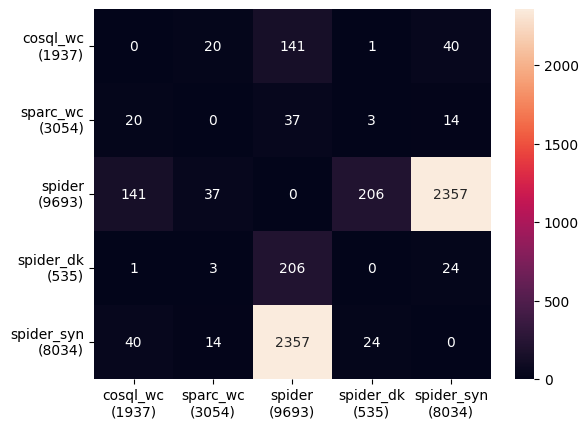
\includegraphics[width=\textwidth]{images/duplicates_before.png}
    \caption{Przed deduplikacją}
    \label{fig:deduplication-before}
\end{subfigure}
\hfill
\begin{subfigure}{0.49\textwidth}
    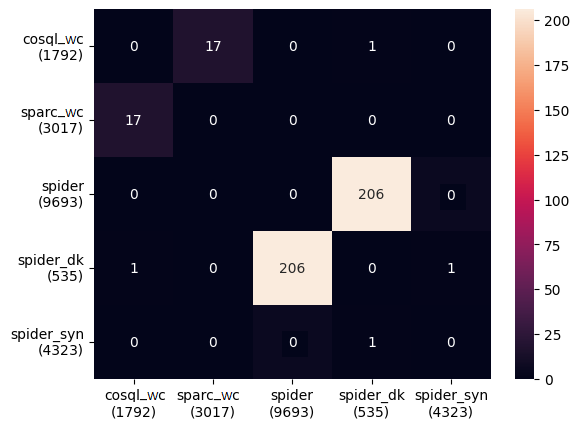
\includegraphics[width=\textwidth]{images/duplicates_after.png}
    \caption{Po deduplikacji}
    \label{fig:deduplication-after}
\end{subfigure}
\caption[Diagramy ilustrujące liczbę duplikatów pomiędzy zbiorami]{Diagramy ilustrujące liczbę duplikatów pomiędzy zbiorami - na osiach umieszczono nazwy zbiorów wraz z liczbą próbek, a wartości w komórkach macierzy wskazują liczbie duplikatów pomiędzy daną parą zbiorów.}
\label{fig:cross-dataset-duplicates}
\end{figure}

\subsubsection{Deduplikacja tłumaczeń}
Deduplikacja tłumaczeń to działanie, które dotyczy wyłącznie zbioru \code{Spider-Syn}. Trzeba zauważyć, że opisane wcześniej usuwania duplikatów bazuje na angielskich wersjach pytań, co wydaję się wystarczające, ponieważ jeżeli pytania angielskie się różnią, to ich polskie tłumaczenia również powinny się różnić. W przypadku próbek zawartych w zbiorze \code{Spider-Syn} jest jednak często inaczej. Dla przypomnienia, zawiera on próbki z oryginalnego zbioru \code{Spider}, lecz z wybranymi słowami zamienionymi na synonimy. Okazuje się, że te synonimy oraz bazowe słowa od których pochodzą tłumaczone są niejednokrotnie przez \code{DeepL} na te same polskie wyrażenia, co skutkuje duplikatami w liczbie 1350. Zostało to przedstawione na rysunku xx. Aby pozbyć się tak powstałej duplikacji postanowiono usunąć niepotrzebne próbki ze zbioru \code{Spider-Syn}. Działanie to, w odróżnieniu do wcześniej opisanych, musiało się odbyć już po dokonaniu tłumaczenia na język polski.

\begin{figure}[ht!]
  \centering
  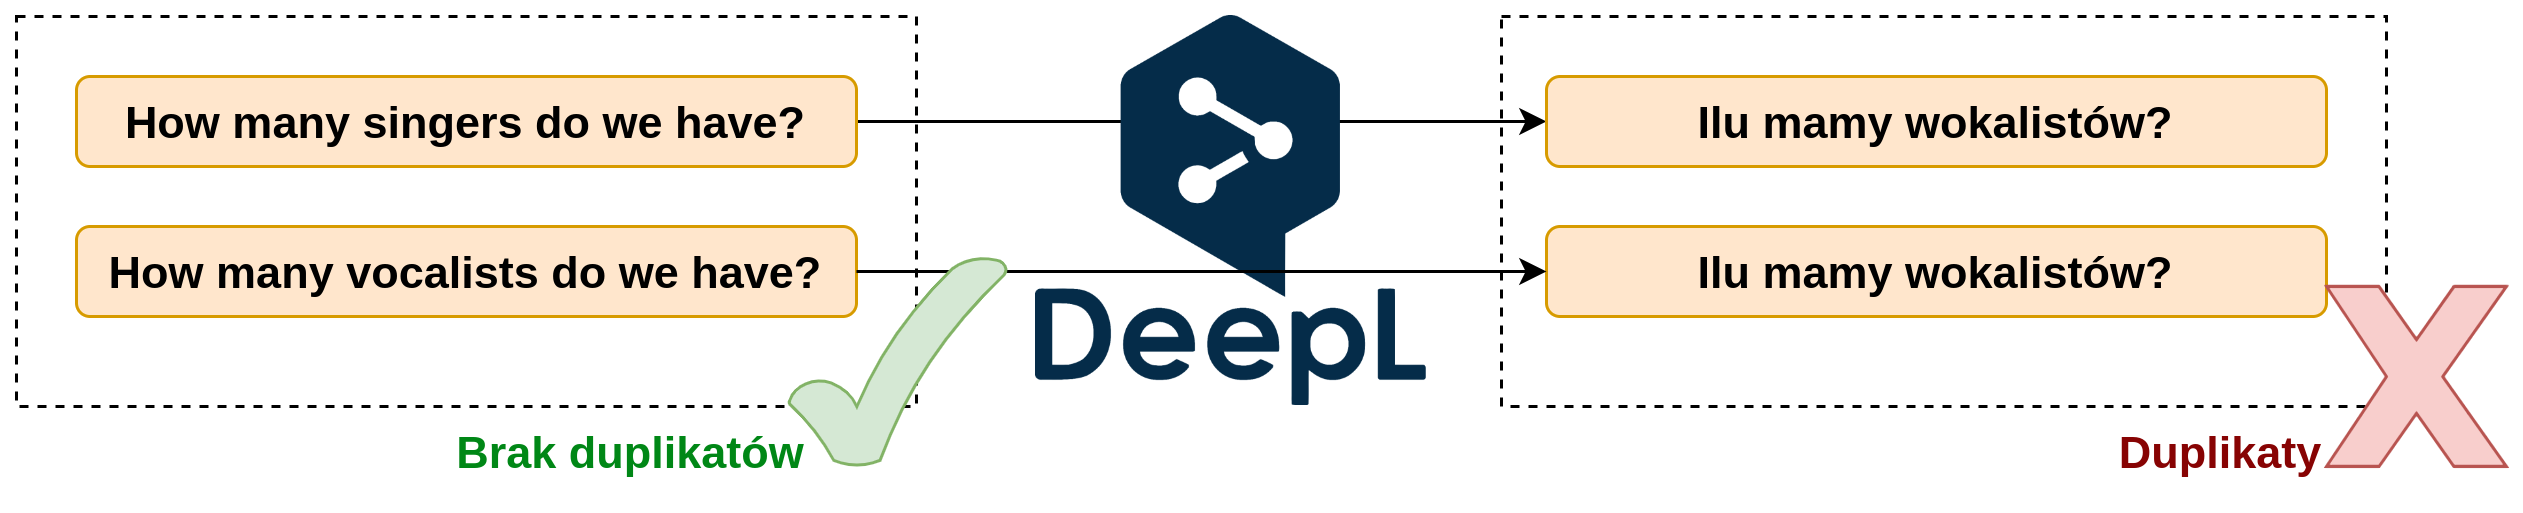
\includegraphics[width=1.0\linewidth]{images/duplication_after_translation.png}
  \caption{Sposób powstawania duplikacji pomiędzy \code{Spider} i \code{Spider-Syn} w wyniku tłumaczenia}
  \label{fig:deduplication_after_translation}
\end{figure}

\section{Dynamiczne generowanie}
Dynamiczne generowanie różnych wariantów zbioru jest ważnym elementem niniejszej pracy i w znaczny sposób odróżnia ją od wcześniejszych podejść. W związku z tym zostanie ono w tej części dokładnie opisane.

Implementacja tej strategii sprowadza się do stworzenia skryptu pozwalającego na wygenerowanie zbioru o żądanych parametrach. Wśród nich możliwe jest określenie języka pytań, języka wartości w zapytaniach i wariantu tłumaczenia schematu bazy danych.

Na początku przedstawione zostaną nowo wprowadzone formaty plików, które stworzony skrypt wykorzystuję do generowania wariantów zbioru.

\subsection{Wprowadzone formaty plików}
W celu umożliwienia generowania różnych wariantów zbioru konieczne było zmodyfikowanie istniejących plików z próbkami poprzez dodanie przetłumaczonych wersji pytań i zapytań SQL oraz opracowany został kompletnie nowy format plików zawierających informację na temat tego jak mają być tłumaczone nazwy tabel i kolumn.

\subsubsection{Format próbek}
Na listingu \ref{lst:new-sample} przedstawiony został format próbek wykorzystany w procesie syntezy zbioru. Porównując ten plik z oryginalnym formatem ze zbioru Spider (przedstawionym wcześniej na listingu \ref{lst:spider-sample}) widać, że zostały dodane polskie odpowiedniki pytań naturalnych oraz zapytań SQL. Nic nie stoi na przeszkodzie dodaniu kolejnego języka, na przykład istniejących już tłumaczeń chińskich lub rosyjskich. W zależności od parametrów podanych do skryptu generującego wybierany jest odpowiedni język. 

\begin{minipage}{\linewidth}
\lstinputlisting[
caption=Fragment pliku \code{tables.json} opisujący schemat pojedynczej bazy danych, label={lst:new-sample}, language=json
]{listings/new_sample.json}
\end{minipage}

Dodatkowo format ten został odchudzony o wszystkie redundantne atrybuty, takie jak tokeny pytania, tokeny zapytania SQL i sparsowane zapytania SQL. Komplikowały one proces tłumaczenia, bo wymagały wprowadzania tych samych zmian w kilku miejscach i narażały zbiór na niespójność. Z tego powodu postanowiono je usunąć z plików zbioru i dodawać dynamicznie podczas jego finalnego generowania.

\subsubsection{Format mapowania nazwy schematu}
Aby umożliwić dokonywanie różnych tłumaczeń schematu baz danych opracowany został format pliku przedstawiony na listingu \ref{lst:new-trans}. Zawiera on informacje pozwalające dokonać mapowania oryginalnych nazw na dowolne inne. Jest to plik json o kilku stopniach zagnieżdżenia. Na najwyższym poziomie jest słownikiem, który dla każdej nazwy bazy zawiera listę tabel, a każda tabela listę kolumn. Wszystkie obiekty reprezentujący tabele i kolumny posiadają docelowe nazwy na jakie powinny zostać przetłumaczone.

\begin{minipage}{\linewidth}
\lstinputlisting[
caption=Fragment pliku zawierającego mapowanie oryginalnych nazw schematu na nowe, label={lst:new-trans}, language=json
]{listings/new_trans.json}
\end{minipage}

Należy zwrócić uwagę, że format ten pozwala, aby dana kolumna była tłumaczona na różne sposoby w zależności od tabeli i bazy w której się znajduję. Podobnie nazwa tabeli może być tłumaczona na różne sposoby w zależności od bazy danych. Jest to celowy zabieg i wymagany w celu umożliwienia wysokiej jakości tłumaczenia. Rozważmy dla przykładu tabelę o nazwie \code{department}. W bazie dotyczącej biznesu prawdopodobnie powinna zostać przetłumaczona jako \code{dział}, natomiast w domenie uniwersyteckiej jako \code{wydział}. Przyjęcie tego bardziej zaawansowanego podejścia umożliwiło dokonanie tłumaczenia kontekstowego, przedstawionego w dalszej części pracy.

\subsection{Zmiana nazw tabel i kolumn}
Dokonanie zmian nazw w schemacie, z punktu widzenia oryginalnego zbioru Spider, sprowadza się do zmodyfikowania dwóch elementów: samych baz danych oraz schematu wewnątrz zapytań SQL. W poniższych sekcjach zostanie przedstawiony opracowany algorytm, który tego dokonuje wraz z analizą alternatywnych możliwości. 

\subsubsection{Modyfikacje w bazach danych}
Zmodyfikowanie nazw tabel i kolumn w bazach danych nie stanowi dużego wyzwania, ponieważ wystarczy wykonać na każdej z nich serię instrukcji typu \sql{ALTER TABLE}. Przystępując do tego należy jednak upewnić się, że zastosowanie danego mapowanie nie tworzy konfliktujących ze sobą pod względem nazw elementów, bo wówczas operacja się nie powiedzie. Podczas tłumaczenia zauważono także, że należy pomijać tabele o nazwie \code{sqlite\_sequence}, ponieważ jest to specjalna tabela i jej modyfikacja nie jest możliwa.

\subsubsection{Modyfikacje w zapytaniach}
Dokonanie podmiany nazw tabel i kolumn w zapytaniach SQL stanowi najtrudniejszy etap w całym procesie generowania zbioru. Przyczyną tego jest przyjęte podejście polegające na tym, że dana kolumna może być przetłumaczona na różne sposoby, w zależności od tabeli w której się znajduję. W przypadku modyfikacji baz danych było oczywistym do której tabeli należy każda kolumna, bo wynika to z ich jasno zdefiniowanej struktury. Zapytania SQL są natomiast w gruncie rzeczy zwykłymi tekstami i wydobycie z nich kolumn oraz ustalenie tabel do których należą stanowi duże wyzwanie.

Najłatwiejsze podejście do tego problemu, ale posiadające istotny problem, wykorzystuje parsowanie zapytań do postaci drzewa AST (ang. Abstract Syntax Tree). Jest to sposób reprezentacji wyrażenia w języku formalnym, takim jak SQL, za pomocą drzewa, którego przykład został przedstawiony na rysunku \ref{fig:ast-example}. Można z niego wygodnie wydobywać różne informacje, czy też dokonywać modyfikacji. Warto więc na jego poziomie przeprowadzić tłumaczenia nazw, a następnie odwrócić proces parsowania i uzyskać dla zapytania zmodyfikowaną postać tekstową. W wykorzystanym języku Python istnieje popularna biblioteka \code{sqlglot}, która pozwala na wykonywanie tego typu operacji. 

\begin{figure}[ht!]
  \centering
  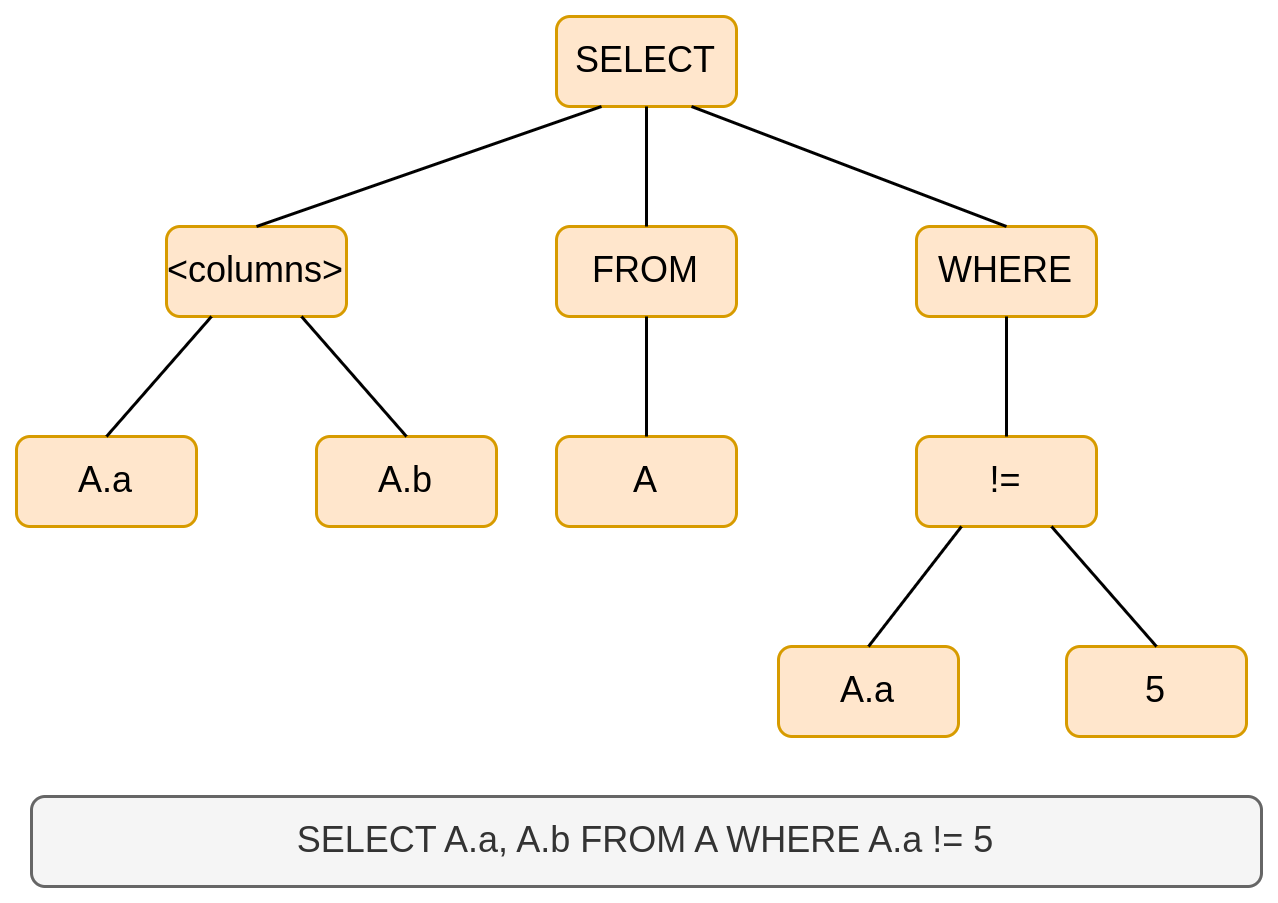
\includegraphics[width=0.6\linewidth]{images/ast_example.png}
  \caption{Drzewo AST dla przykładowego zapytania SQL}
  \label{fig:ast-example}
\end{figure}

Wspomnianym problemem z wykorzystaniem AST jest to, że przetłumaczone z wykorzystaniem biblioteki \code{sqlglot} zapytania, chociaż pod względem semantycznym pozostają bez zmian, to modyfikacji ulega ich formatowanie - następuje zmiana sposobu nawiasowania, czy też stawiania białych znaków. Przekonwertowane w ten sposób zapytania odbiegają więc istotnie od oryginalnych i porównywanie takiego zbioru z oryginalnym \code{Spider} mogło by być kwestionowane. Ponadto wiele algorytmów opiera się na specyficznym dla zbioru \code{Spider} formacie zapytań i jego modyfikacja doprowadziła by do problemów z uruchomieniem wielu modeli. Z przytoczonych powodów porzucono to podejście.

W celu dokonania modyfikacji schematu w zapytaniach, bez niepotrzebnego wpływania na ich strukturę, zdecydowano się ostatecznie zrobić to na niższym poziomie. W tym celu opracowano algorytm, który najpierw dokonuje tokenizacji zapytań, a następnie analizuje wszystkie tokeny po kolei i jeżeli trafi na nazwę kolumny lub tabeli to dokonuję podmiany na nową nazwę. Aby sprawdzić, czy dany token jest nazwą kolumny lub tabeli dokonywano parsowania zapytania do AST, następnie zmieniano dany token na inny i ponownie parsowano zapytanie do AST. Porównując ze sobą te dwa drzewa AST można było ustalić, czy zmodyfikowanym tokenem była nazwa tabeli, nazwa kolumny, czy żadne z powyższych.

W celu przetłumaczenia nazwy kolumny należało dodatkowo ustalić, do jakiej tabeli ona należy. Aby to zrobić konieczne było rozpatrzenie trzech możliwych przypadków:

\begin{enumerate}
    \item Nazwa kolumny poprzedzona nazwą tabeli (\sql{SELECT order.id FROM order})
    \item Nazwa kolumny poprzedzona aliasem (\sql{SELECT T1.id FROM order as T1})
    \item Nazwa kolumny bez tabeli (\sql{SELECT id FROM order})
\end{enumerate}

Pierwszy scenariusz jest najprostszy, ponieważ nazwa tabeli jest jawnie podana i nie ma co do niej wątpliwości. Drugi przypadek jest bardziej skomplikowany ponieważ zamiast istniejącej nazwy tabeli wykorzystany został stworzony alias, więc wcześniej trzeba wydobyć z zapytania wszystkie aliasowania. Trzeci przypadek jest również trudny, ponieważ kolumna należy do jednej z wykorzystanych w zapytaniu tabel, więc trzeba wiedzieć dodatkowo jakie tabele są dostępne. Dla tych dwóch przypadków sytuację dodatkowo komplikuję fakt, że zapytania mogą być swobodnie zagnieżdżanie i łączone szeregowo za pomocą operatorów zbiorowych, co skutkuje tym, że w obrębie pojedynczego zapytania pojawiają się zakresy w których dostępne są różne tabele i różne aliasowania.

Aby poradzić sobie z ustaleniem przynależności kolumn do tabel w skomplikowanych zapytaniach postanowiono więc dokonywać rekurencyjnego rozbijania składających się na nie tokenów, przekazując przy tym kontekst mówiący o obowiązującym aliasowaniu z zapytań nadrzędnych do podrzędnych. Zostało to zilustrowane na rysunkach 
\ref{fig:query-decomposition-serial} oraz \ref{fig:query-decomposition-nested}. Przedstawiają one odpowiednio dekompozycję zapytania zawierającego operator zbiorowy oraz dekompozycję zapytania z zagnieżdżeniem. W tym drugim przypadku miejsce zapytania podrzędnego jest zastępowane poprzez fragment \sql{SELECT 1}, aby zapewnić strukturalną poprawność obu wynikowych zapytań. W wyniku tego procesu otrzymywany jest zbiór elementarnych zapytań wraz z obowiązującymi wewnątrz nich kontekstami, co pozwala na łatwą modyfikację tokenów odpowiadających za nazwy tabel i kolumn. Jako, że pierwotnym źródłem tych tokenów jego wejściowe, skomplikowane zapytanie to również ono jest tłumaczone - niejako jako efekt uboczny, lecz jest to celowym zamierzeniem.

% Podczas tego procesu kontekst z zapytań nadrzędnych, jest przekazywany do zapytań podrzędnych, aby utrzymywać przez cały czas informację o dostępnych w danej części zapytania aliasowaniach.

\begin{figure}[ht!]
  \centering
  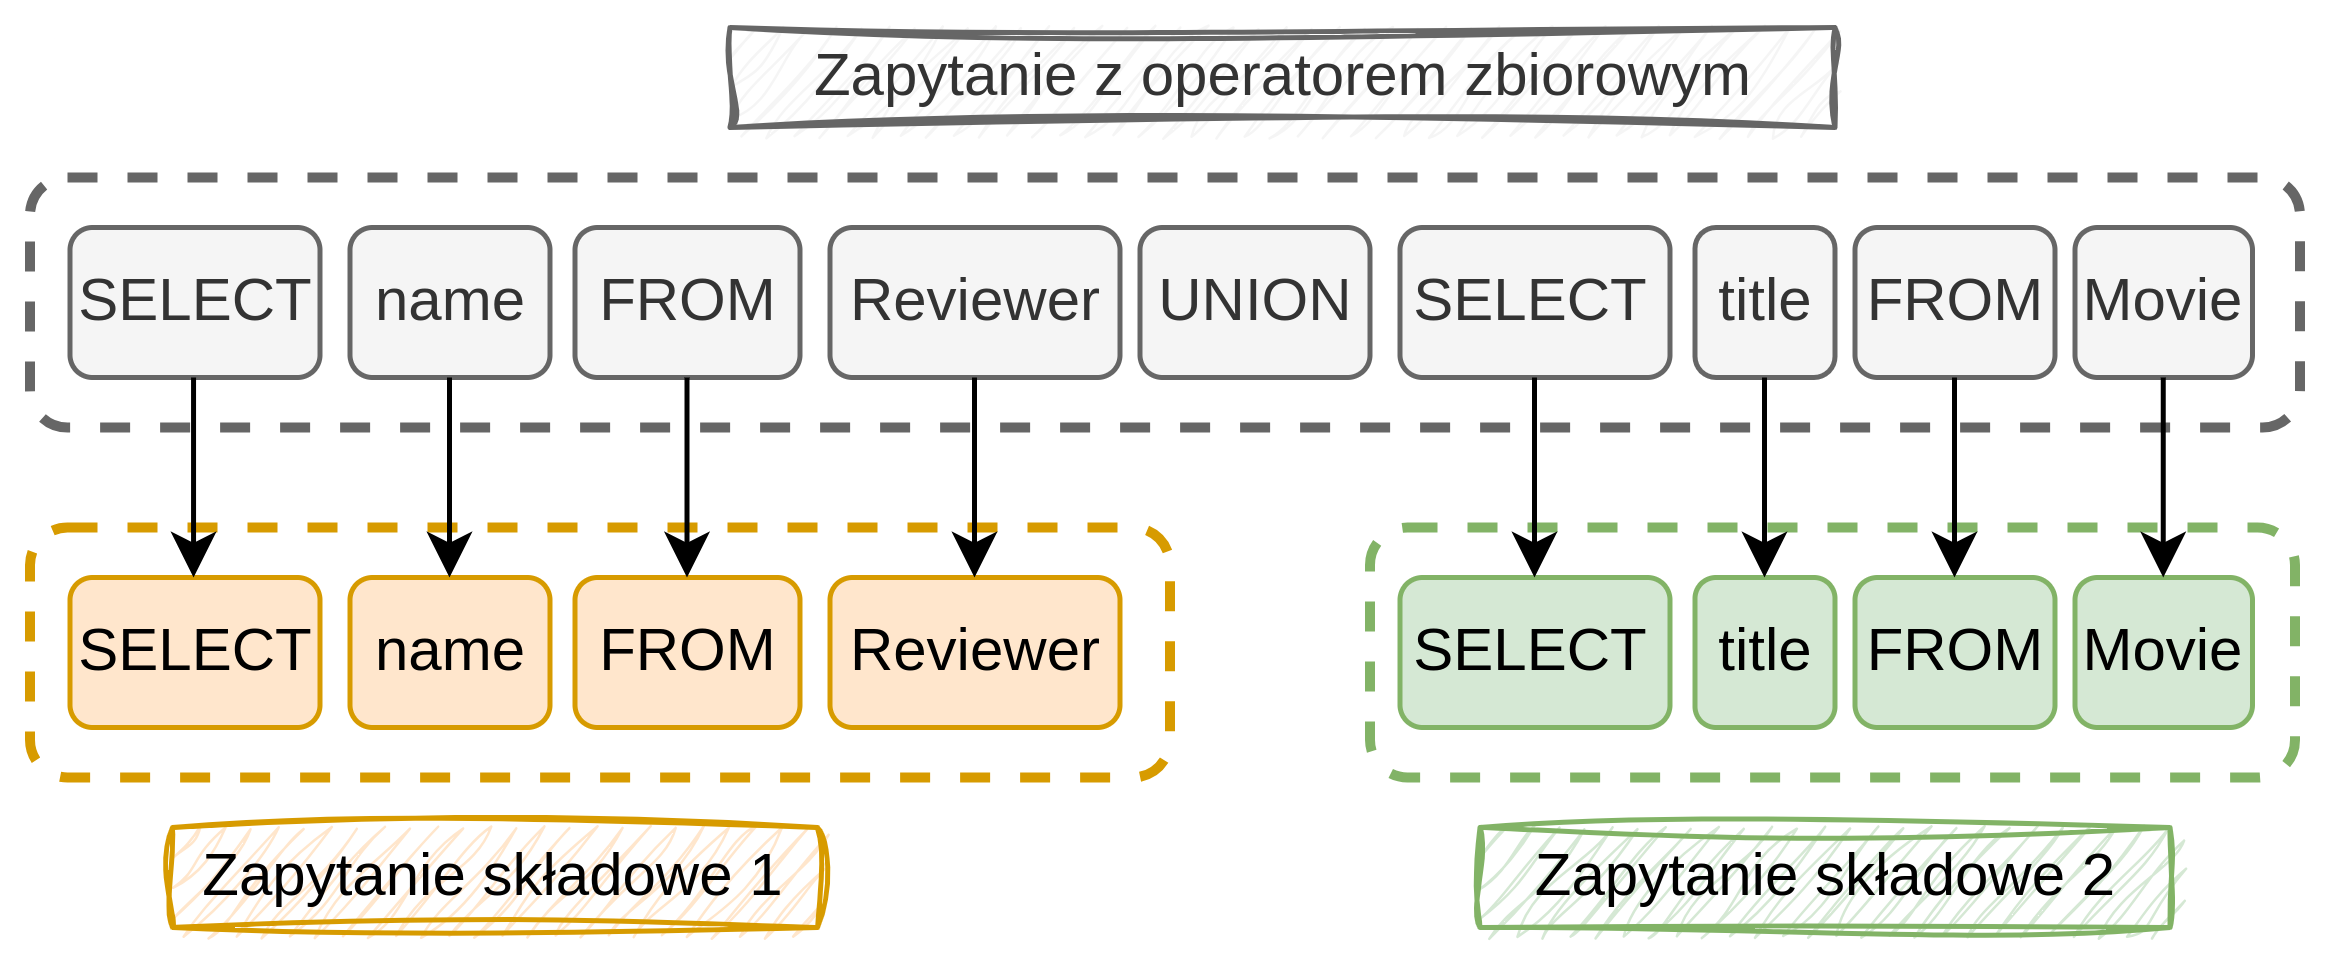
\includegraphics[width=1.0\linewidth]{images/query_decomposition_serial.png}
  \caption{Metoda dekomponowania zapytań z operatorami zbiorowymi}
  \label{fig:query-decomposition-serial}
\end{figure}

\begin{figure}[ht!]
  \centering
  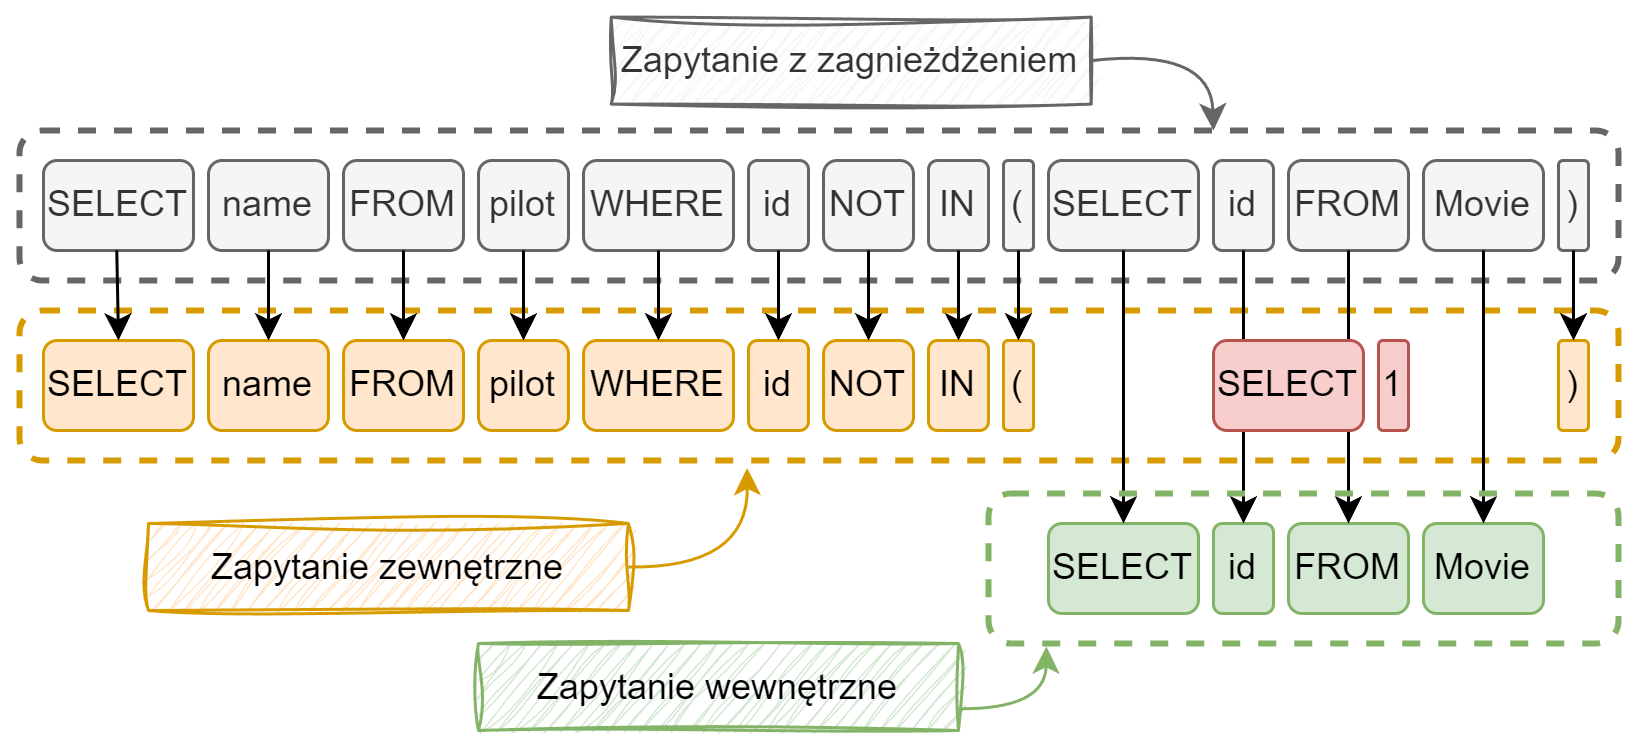
\includegraphics[width=1.0\linewidth]{images/query_decomposition_nested.png}
  \caption{Metoda dekomponowania zapytań zagnieżdżonych}
  \label{fig:query-decomposition-nested}
\end{figure}

\subsection{Dodawanie informacji redundantnych}
Jak zostało wcześniej wspomniane i zademonstrowane na listingach z źródłowych danych wykorzystywanych do generowania finalnego zbioru zostały usunięte informacje redundantne, aby umożliwić łatwiejsze wprowadzanie modyfikacji. W procesie ostatecznej syntezy należy jednak te informacje ponownie odtworzyć, aby stworzony zbiór w żaden sposób nie odbiegał formatem od oryginalnego.

Dużą część dodatkowych informacji stanowią pytania oraz zapytania SQL podzielone na tokeny. Okazuję się, że duża część istniejących rozwiązań nie wykorzystuje tych informacji, ponieważ tokenizacji można dokonać na różne sposoby i wiele rozwiązań wykonuję ją samodzielnie, wybierając sposób dla siebie najkorzystniejszy. Nie mniej jednak pierwsze modele, jak i zapewne część nowszych, korzysta z dostarczonego w ramach zbioru sposobu tokenizacji, więc należy o ten aspekt zadbać.

\subsubsection{Tokenizacja pytań}
Pytania podzielone na tokeny występują w próbkach pod kluczem \code{question\_toks}. Tokenizacji postanowiono dokonać za pomocą dostarczonego w ramach biblioteki \code{spaCy} wielojęzycznego modelu. Wybrano akurat model wielojęzyczny, a nie polski, ponieważ założono, że tworzony skrypt ma mieć możliwość generowania w razie potrzeby zbiorów z pytaniami angielskimi. Porównano jednocześnie rezultaty tokenizacji polskich pytań za pomocą modelu wielojęzycznego oraz polskiego. Okazuję się, że wyniki różnią się jedynie w niewielkiej liczbie przypadków, co świadczy o tym, że model wielojęzyczny jest dość wysokiej jakości.

\subsubsection{Tokenizacja zapytań SQL}
Kolejnym elementem, który trzeba dodać do wynikowego zbioru są zapytania SQL podzielone na tokeny. Występują one wewnątrz próbek pod kluczem \code{question\_toks}. Zaimplementowany sposób tokenizacji głównie opiera się na podzieleniu zapytań SQL na poszczególne elementy składowe, takie jak słowa kluczowe \sql{SELECT}, \sql{FROM}, \sql{WHERE}, czy nazwy tabel i kolumn. Wyjątkiem są występujące wewnątrz zapytań wartości tekstowe, które dzielone są na tokeny przy pomocy wielojęzycznego modelu z biblioteki \code{spaCy}, wspomnianego przy okazji omawiania tokenizacji pytań. Opisany proces został zilustrowany na rysunku \ref{fig:query-tokenization}.

\begin{figure}[ht!]
  \centering
  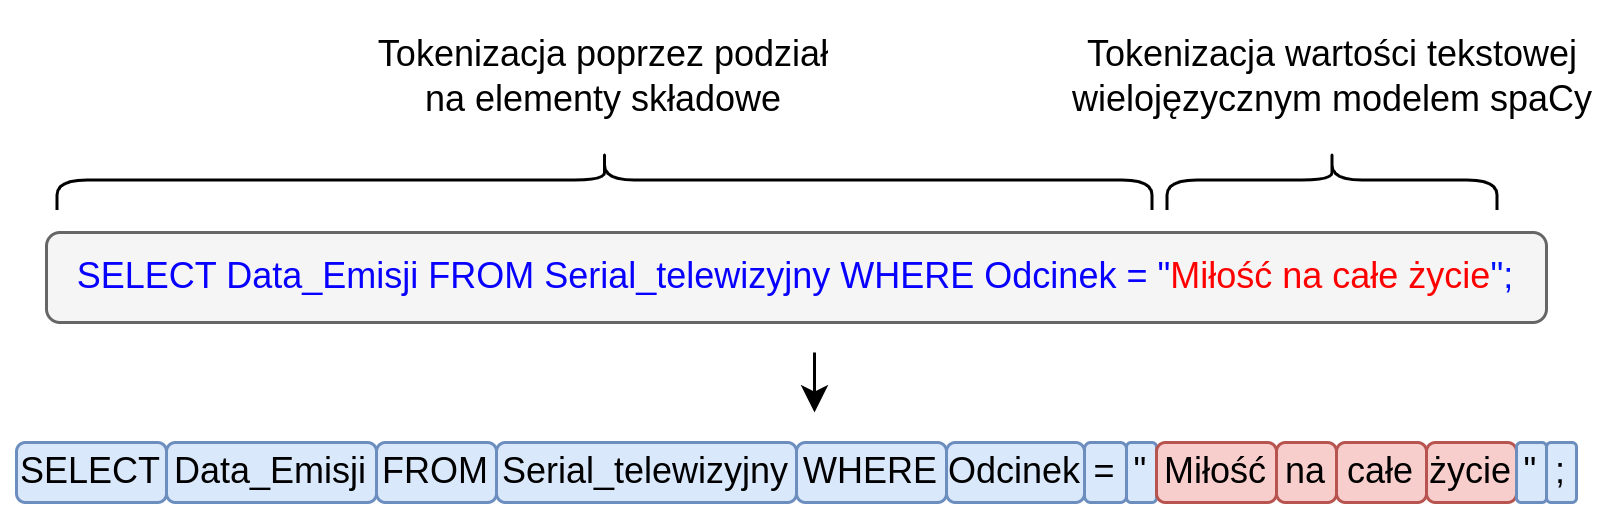
\includegraphics[width=1.0\linewidth]{images/query_tokenization.png}
  \caption{Schemat zaimplementowanej strategii tokenizacji zapytań SQL}
  \label{fig:query-tokenization}
\end{figure}

\subsubsection{Tokenizacja zapytań SQL bez wartości}
Próbki w zbiorze \code{Spider} posiadają także atrybut o nazwie \code{query\_toks\_no\_value}, który powinien zawierać zapytanie SQL podzielone na tokeny, ale bez wartości, a dokładnie wartości powinny zostać zamaskowane za pomocą specjalnego tokena \code{value}. Została więc wykorzystana ta sama technika co do standardowej tokenizacji zapytań, lecz dodatkowo wszystkie wartości zostały znalezione z wykorzystaniem biblioteki \code{sqlparse} i zamaskowane.

Opracowany algorytm jest niemal całkowicie zbieżny z wykorzystanym w oryginalnym zbiorze \code{Spider} sposobem tokenizacji. Aby to zweryfikować za jego pomocą dokonano tokenizacji oryginalnych zapytań i sprawdzono, czy wyniki pokrywają się z oryginalnymi tokenami. Okazuję się, że różnice występują jedynie w 18 przypadkach spośród prawie dziesięciu tysięcy. Sposób tokenizacji tych kilkunastu oryginalnych zapytań wyraźnie odbiega od całej reszty i przypuszcza się, że jest to niespójność oryginalnego zbioru. 

\subsubsection{Parsowanie zapytań SQL}
Ostatnim elementem, który należy dodać do zbioru są sparsowane zapytania SQL, występujące w próbkach pod kluczbem \code{sql}. Tym razem istnieje publicznie dostępny skrypt, który dokonuje tego procesu. Zostały napotkane jednak pewne problemy wynikające z jego niedociągnięć. W jednym z pierwszych kroków dokonuje on wydobycia z zapytania aliasowania, czyli słownika mówiącego jakie występują w nim aliasy i na jakie tabele się mapują. Niestety dokonuje tego globalnie, a jak zostało przedyskutowane wcześniej, nie sprawdzi się to dla wszystkich zapytań, ponieważ występują w nich zakresy - w jednej części zapytania dany alias może mapować się na zupełnie inną tabelę niż w drugiej części. Podczas uruchamiana tego skrypt na zapytaniach ze zbioru \code{Spider} (co jest najczęstszym scenariuszem jego wykorzystania) nie zwraca on żadnych błędów. Przypuszcza się, że kłopotliwe zapytania zostały ręcznie poprawione, by stały się parsowalne. W przypadku jednak, gdy zapytania zostaną wcześniej poddane tłumaczeniu nazw schematu, to problem ten wychodzi na wierzch i parsowanie kończy się najczęśniej dla kilku zapytań niepowodzeniem. 

Nasuwające się rozwiązania powyższego problemu są dwa: można poprawić skrypt parsujący lub zmodyfikować tłumaczenia tak, aby problem się nie ujawnił. Postanowiono wybrać drugą opcję, ponieważ nie wymaga ona wiele wysiłku w odróżnieniu do skomplikowanej naprawy skryptu. Przypuszcza się, że podobny był również sposób myślenia twórców zbioru \code{Spider} - zaimplementowali uproszczony skrypt parsujący, ponieważ koszt zaimplementowania wariantu pełnego znacznie przewyższa koszt jednorazowego dostosowania kilkudziesięciu zapytań. Nie mniej jednak zauważone zachowanie zostało zgłoszone na platformie \code{GitHub} w odpowiednim repozytorium, by udokumentować i zwrócić uwagę na tą kwestię.

\section{Wykonywanie tłumaczenia}
Jeden podrozdział opisywał format źródłowych danych, a kolejny sposób generowania na ich podstawie finalnych zbiorów. Nie została jeszcze poruszona kwestia tego w jaki sposób otrzymywane są znajdujące się w tych danych źródłowych tłumaczenia, poza przyjętym założeniem co do tłumaczenia maszynowego - zostanie to przedstawione w tej części.

\subsection{Wybór tłumacza}
Ważną do podjęcia decyzją był wybór konkretnego narzędzie mającego być wykorzystanym do tłumaczenia maszynowego. Obecnie większość tego typu rozwiązań bazuje na uczeniu głębokim. Są one zazwyczaj zastrzeżone i dostęp do nich uzyskuje się za pomocą webowego API. Istnieją również narzędzia typu \code{open source}, które można uruchomić w całości na własnym urządzeniu. Pozwalają uniknąć naliczania kosztów i dają możliwość swojej modyfikacji. Oferują za to mniejszą dokładność i dlatego postanowiono zrezygnować z tej drogi.

Podczas podejmowania ostatecznej decyzji wybór ograniczono do popularnych i renomowanych rozwiązań, takich jak \code{Google Cloud Translation API} \cite{google-translation-api}, \code{Microsoft Azure AI Translator} \cite{microsoft-translator}, \code{Amazon Translate API} \cite{amazon-translator} oraz \code{DeepL} \cite{deepl}. W szczególności to ostatnie wydaje się aktualnie wychodzić na prowadzenie pod względem jakości produkowanych tłumaczeń. Według informacji zawartych na swojej stronie \code{DeepL} generuje tłumaczenia ponad 3 razy dokładniejsze od rozwiązań konkurencji. Wysoką ich jakość potwierdzają również liczne artykuły naukowe \cite{Yulianto2021}\cite{Ternero2021}\cite{Bahasa2023}, które powstały na fali zachwytu tym rozwiązaniem. Posiada nawet dedykowaną bibliotekę do języka \code{Python}, ułatwiającą jego wykorzystanie. 

Jedynym aspektem, który może zniechęcać do wykorzystania \code{DeepL} są związane z tym koszty. W czasie tworzenia niniejszej pracy podstawowy plan opierał się na bazowej opłacie w kwocie 20 złotych na miesiąc oraz dodatkowym obciążeniu wynoszącym prawie 90 złotych za każdy przetłumaczony milion znaków. Dostępny jest jednak również darmowy plan, pozwalający na przetłumaczenie pół miliona znaków każdego miesiąca za darmo.

To właśnie \code{DeepL} zostało ostatecznie wybranym narzędziem, a głównym tego powodem jest niekwestionowana jakość produkowanych przez nie tłumaczeń. Oszacowano, że dostępne w ramach darmowego planu limity powinny pozwolić na zrealizowanie postawionych celów. Nie uda się to jednak w jeden miesiąc, a konieczne będzie rozłożenie tłumaczeń na dłuższy okres.

\subsection{Tłumaczenie nazw tabel i kolumn}
Okazuje się, że tłumaczenie nazw tabel i kolumn jest trudnym zadaniem i z tego powodu zostało ono podzielone na dwa etapy. Pierwszy zakłada wykorzystanie tłumacza maszynowego, a drugi ręczne poprawienie tłumaczeń. W tym przypadku to ostatnie nie polega jednak na przeglądaniu każdego tłumaczenia jedno po drugim, lecz na bardziej heurystycznym podejściu, które zostanie dokładniej opisane.

\subsubsection{Tłumaczenie maszynowe}
Jako zostało wcześniej zaznaczone, w zbiorze \code{Spider} dla tabel i kolumn występują podwójne nazwy: oryginalnie występujące w bazie danych (\code{first\_name}) oraz w czytelnej, naturalnej postaci (\code{first name}). O ile przetłumaczenie tych ostatnich nie stanowi większego problemu, to nazwy oryginalne wymagają podjęcia dodatkowych akcji, ponieważ \code{DeepL} nie poradzi sobie z nimi w tej postaci - jako tłumaczenie zwróci te same nazwy, bez dokonywania żadnych zmian (\code{first\_name}), ponieważ potraktuje je jako nazwy własne, które nie podlegają tłumaczeniu. Zauważono, że \code{Google Cloud Translation} wykazuję pod tym kątem bardziej pożądane zachowanie, ale wciąż nie można by było na nim polegać. 

Aby poradzić sobie z zarysowanym problemem postanowiono przed tłumaczeniem dokonywać w nazwach podmiany znaków podkreślenia na spacje, by przekonwertować je do postaci naturalnej, a po tłumaczeniu spacje z powrotem zamieniać na znaki podkreślenia, co przedstawione zostało na rysunku \ref{fig:multi-word-translation}. Mechanizm ten nie sprawdził się dla wszystkich przypadków, ponieważ niektóre wielowyrazowe nazwy były zapisywane za pomocą innych konwencji niż oddzielanie słów znakiem podkreślenia. Były one jednak w mniejszości i tymi niedociągnięciami postanowiono się zająć na etapie ręcznych poprawek.

\begin{figure}[ht!]
  \centering
  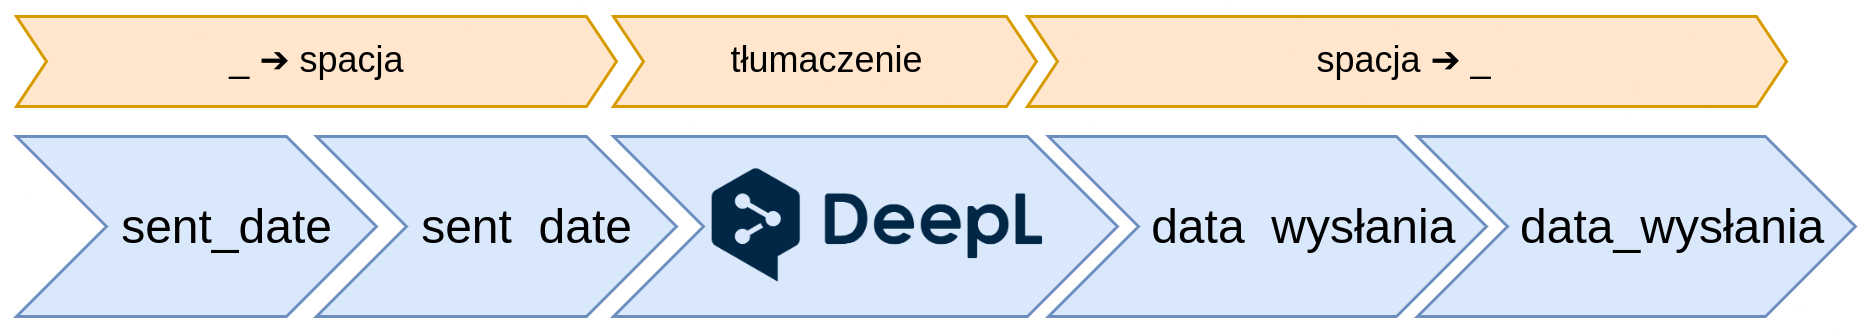
\includegraphics[width=1.0\linewidth]{images/multi_word_translation.png}
  \caption{Schemat algorytmu do tłumaczenia oryginalnych nazw tabel i kolumn}
  \label{fig:multi-word-translation}
\end{figure}

Podstawowa metoda tłumaczenia nazw to ich proste i intuicyjne przekazywanie do tłumacza. Jest to sposób, który został prawdopodobnie wykorzystany we wszystkich tłumaczeniach maszynowych zbioru \code{Spider}, ponieważ ich autorzy nie zwrócili szczególnej uwagi na tą kwestię. Podczas realizacji niniejszej pracy zauważono jednak, że wiele błędów w takich tłumaczeniach wynika z braku uwzględniania przez tłumacza kontekstu i opracowano metodę, która pozwala w dużej mierze obejść ten problem. Dla przykładu kolumna \code{home\_games}, podstawową metodą jest tłumaczona jako \code{gry\_domowe}, natomiast ulepszona metoda kontekstowa weźmie pod uwagę, że kolumna znajduję się w tabeli \code{stadium} oraz bazie danych \code{game\_injury} i tym razem nazwa zostanie przetłumaczona jako \code{mecze\_u\_siebie}.

Metoda kontekstowa polega na obserwacji, że nowoczesne narzędzia bazujące na sieciach neuronowych, w szczególności \code{DeepL}, tłumaczą to samo słowo w różny sposób w zależności od kontekstu w jakim ono wystąpiło. Z tego powodu do tłumacza poza samymi nazwami tabel i kolumn postanowiono także podawać w roli kontekstu nazwy baz danych, a dla kolumn również nazwy tabeli. Zostały opracowane szablony, które służą do tworzenia skontekstualizowanych wyrażeń podawanych do tłumacza i wraz z przykładami użycia zostały przedstawione na rysunku \ref{fig:translation-in-context}. Dla porównania postanowiono dokonać tłumaczenia bezkontekstowego i okazało się, że wynikowe tłumaczenia nazw pomiędzy tymi metodami różnią się dla 21,41\% przypadków, co stanowi dużą różnicę.

\begin{figure}[ht!]
\centering
\begin{subfigure}{0.4\textwidth}
    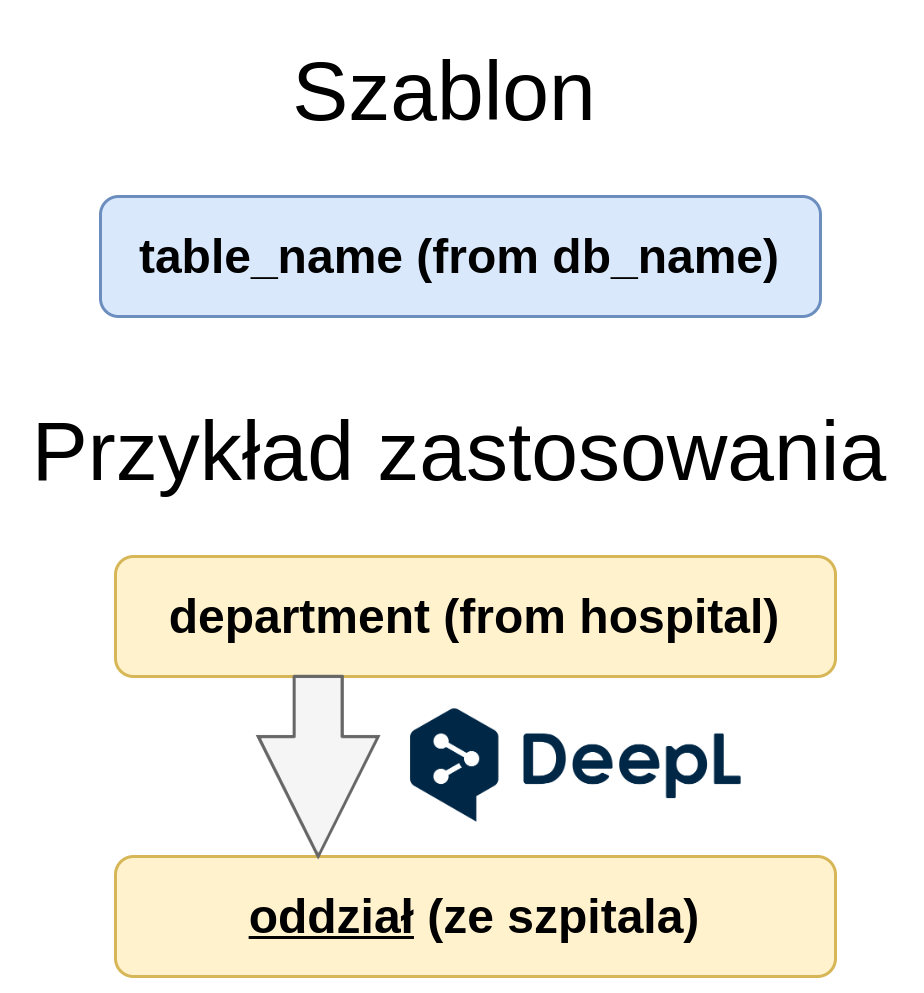
\includegraphics[width=\textwidth]{images/translation_in_context_table.png}
    \caption{Dla tabel}
    \label{fig:first}
\end{subfigure}
\hfill
\begin{subfigure}{0.50\textwidth}
    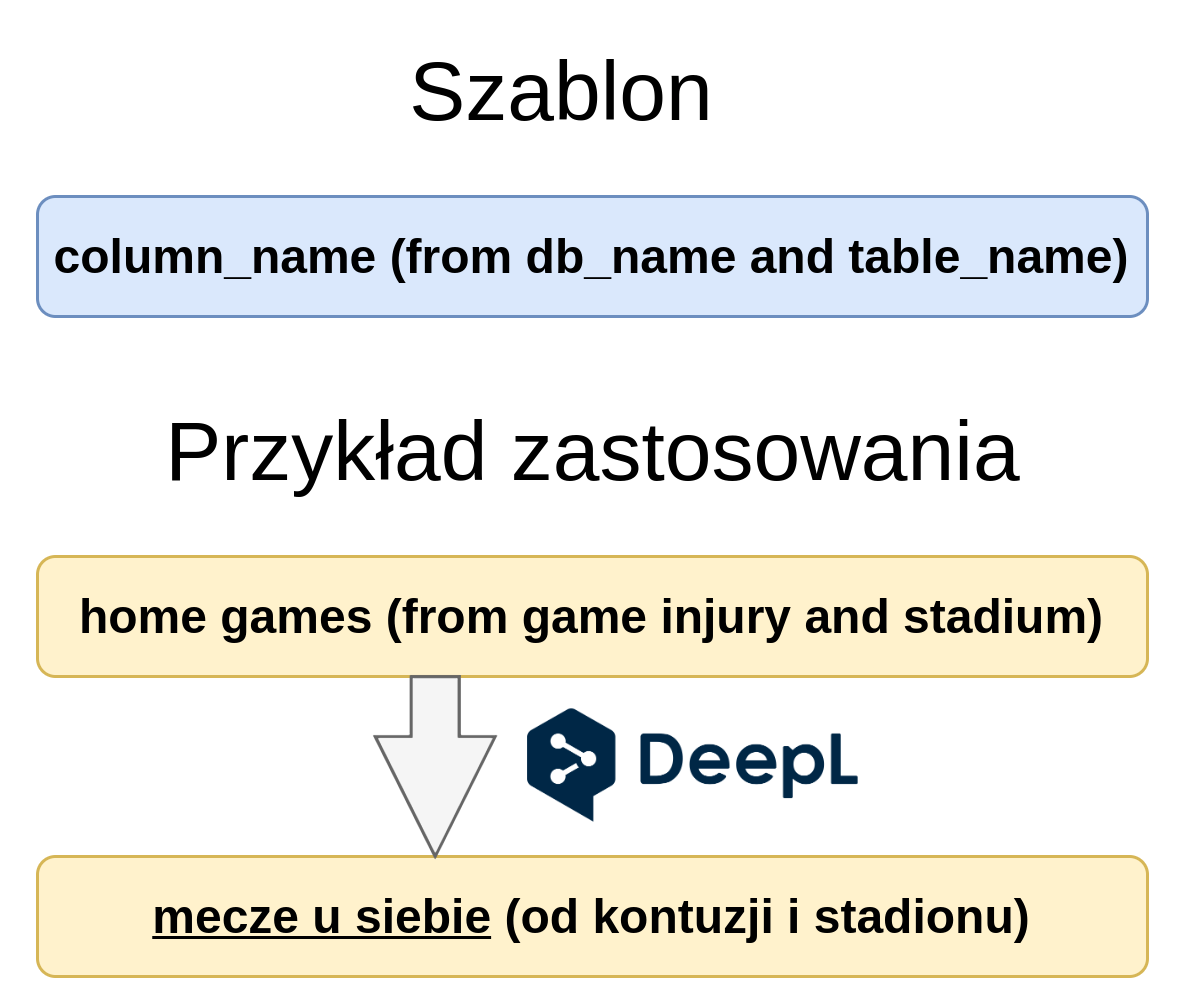
\includegraphics[width=\textwidth]{images/translation_in_context_column.png}
    \caption{Dla kolumn}
    \label{fig:second}
\end{subfigure}
\caption{Szablony do tłumaczenia kontekstowego}
\label{fig:translation-in-context}
\end{figure}

Przedstawiona strategia tłumaczenia kontekstowego jest zainspirowana metodą \code{SAVe}, opisaną w artykule dotyczącym wielojęzycznego zbioru \code{MultiSpider} \cite{Dou2022}. Została tam wykorzystana jako metoda augmentacji w celu poprawienia osiąganych przez model wyników. Jest bardziej skomplikowana od przedstawionego powyżej wariantu, ponieważ zakłada wykorzystanie wielu szablonów oraz ma dodatkowych etap weryfikacji tłumaczeń, co jednak dla rozważanego problemu nie ma dobrego uzasadnienia.

Oczywistym minusem zaproponowanej metody jest istotne zwiększenie długości tekstów podawanych do tłumacza, co w przypadku \code{DeepL} wpływa na naliczenie wyższych kosztów lub też szybsze wykorzystanie darmowych limitów - na co się mimo wszystko zdecydowano. Zaletą strategii kontekstowej jest poprawa tłumaczenia dla wielu nazw, jednak z pewnego punktu widzenia może ona także wpływać na obniżenie czytelności przetłumaczonego schematu. Zdarzają się bowiem przypadki, iż w obrębie jednej bazy pewna nazwa kolumny zostaje przetłumaczona na kilka różnych sposobów, chociaż nie powinna. Zmniejsza to spójność tak przetłumaczonego schematu, bo sugeruje, że przechowywane są w tych kolumnach dane o różnym znaczeniu, a w rzeczywistości jest inaczej. Nie jest więc banalnym oszacowanie wypadkowego wpływu zastosowania tej metody na jakość finalnego zbioru, uważa się jednak, że jest on pozytywny.

\subsubsection{Ręczne poprawki}
Po uzyskaniu tłumaczeń maszynowych nazw tabel i kolumn oraz ich wstępnej ocenie było oczywistym, że wciąż zawierają pewne błędy. Przejrzenie każdego z nich jedno po drugim wymagałoby znacznego nakładu czasu, więc postanowiono posłużyć się metodami heurystycznymi, by zlokalizować tylko te najbardziej podejrzane. 

Zauważono, że dla błędnych tłumaczeń bardzo często nazwa przetłumaczona jest identyczna z angielską, więc korzystając z tego faktu, prostych skryptów oraz możliwości edytora \code{Visual Studio Code} dokonano znalezienia właśnie takich przypadków, a następnie je poprawiono. Były to w dużej mierze nazwy składające się z kilku wyrazów połączonych ze sobą za pomocą innej konwencji niż znaki podkreślenia, bo tylko ten najpopularniejszy wariant był obsługiwany w fazie maszynowej. Dość częste były również kilkuliterowe skróty jak \code{mid} (movie id), czy \code{aid} (author id), z którymi - co nie dziwi - \code{DeepL} sobie nie poradził. Poza tym dokonano poprawy kilkunastu wyrażeń w przypadku których zaobserwowano częste pomyłki, jak tłumaczenie \code{name} na \code{imię i nazwisko}, chociaż powinno zostać przetłumaczone jako \code{nazwa}, czy \code{id}, które niepotrzebnie zostało przetłumaczone na rozwlekłą nazwę \code{identyfikator}.

Na cały etap ręcznych poprawek zostało poświęcone kilka godzin i w jego wyniku zmodyfikowanych zostało 10,54\% tłumaczeń maszynowych. Wydaje się to dużą częścią, lecz większość z tych modyfikacji dokonano w szybki, półautomatyczny sposób.


\subsection{Tłumaczenie pytań}
Tłumaczenie pytań sprowadza się do uzupełnienia w przedstawionym wcześniej formacie próbek wartości \code{question.pl} na podstawie atrybutu \code{question.en}. W tym przypadku pytania zostały bezpośrednio przekazane do tłumacza, bez stosowania żadnych dodatkowych sztuczek. Uznano, że stosowanie tłumaczenia kontekstowego, które oznaczałoby rozszerzenie przekazywanych do tłumacza tekstów o nazwę bazy danych z której pochodzą, nie ma sensu. Wiązałoby się to z tłumaczeniem większej liczby znaków na podstawie których \code{DeepL} obciąża swoich użytkowników, a uzyskana poprawa prawdopodobnie nie byłaby znacząca. Pytania są bowiem zwykle na tyle długie, że pozwalają tłumaczowi na wywnioskowanie domeny której dotyczą i wybranie odpowiednich tłumaczeń dla problematycznych słów. 

Etap manualnych poprawek nie został w tym przypadku wykorzystany, gdyż pytania zawierają dużą ilość tekstu i ciężko jest dostrzec w nich ewentualne błędy. Nie znaleziono również żadnych sposobów na znalezienie podejrzanych tłumaczeń, czy dokonanie półautomatycznych poprawek, tak jak to miało miejsce dla tłumaczenia nazw tabel i kolumn. Ostatecznie maszynowe tłumaczenia pytań wydawały się na tyle wysokiej jakości, że postanowiono przejść do kolejnych etapów.

\subsection{Tłumaczenie wartości w zapytaniach SQL}
Tłumaczenie wartości w zapytaniach SQL odbyło się poprzez uzupełnienie atrybutów \code{query.pl} na podstawie \code{query.en} w pliku z próbkami o przedstawionym wcześniej formacie. Ten ostatni atrybut zawiera oryginalne zapytania SQL, natomiast pierwszy zapytania z wszelkimi anglojęzycznymi łańcuchami znaków przetłumaczonymi na język polski.

W celu znalezienia w danym zapytaniu wartości tekstowych dokonywano jego przetwarzania z wykorzystaniem biblioteki \code{sqlparse}. Pozwalała ona podzielić zapytanie na poszczególne tokeny i wybrać te, które posiadają typ \code{Token.Literal.String}, czyli właśnie wartości tekstowe. Są to wyrażenia zamknięte w pojedynczych lub podwójnych cudzysłowach, które przekazywano do \code{DeepL} w celu uzyskania tłumaczeń, a następnie zastępowano nimi oryginalne teksty. Wyjątek stanowią jedynie wartości występujące w roli szablonów po słowie kluczowym \code{LIKE}, takie jak \code{'\%Hey\%'}, \code{'\%East\%'}, \code{'S\%'}. Nie są one zapisane w języku naturalnym, ponieważ zawierają specjalne znaki, stanowiące problem dla tłumacza maszynowego. Z tego względu, a także biorąc pod uwagę rzadkość takich przypadków, postanowiono przetłumaczyć je manualnie. Wizualizacja tego etapu została przedstawiona na rysunku \ref{fig:value-translation}

\begin{figure}[ht!]
  \centering
  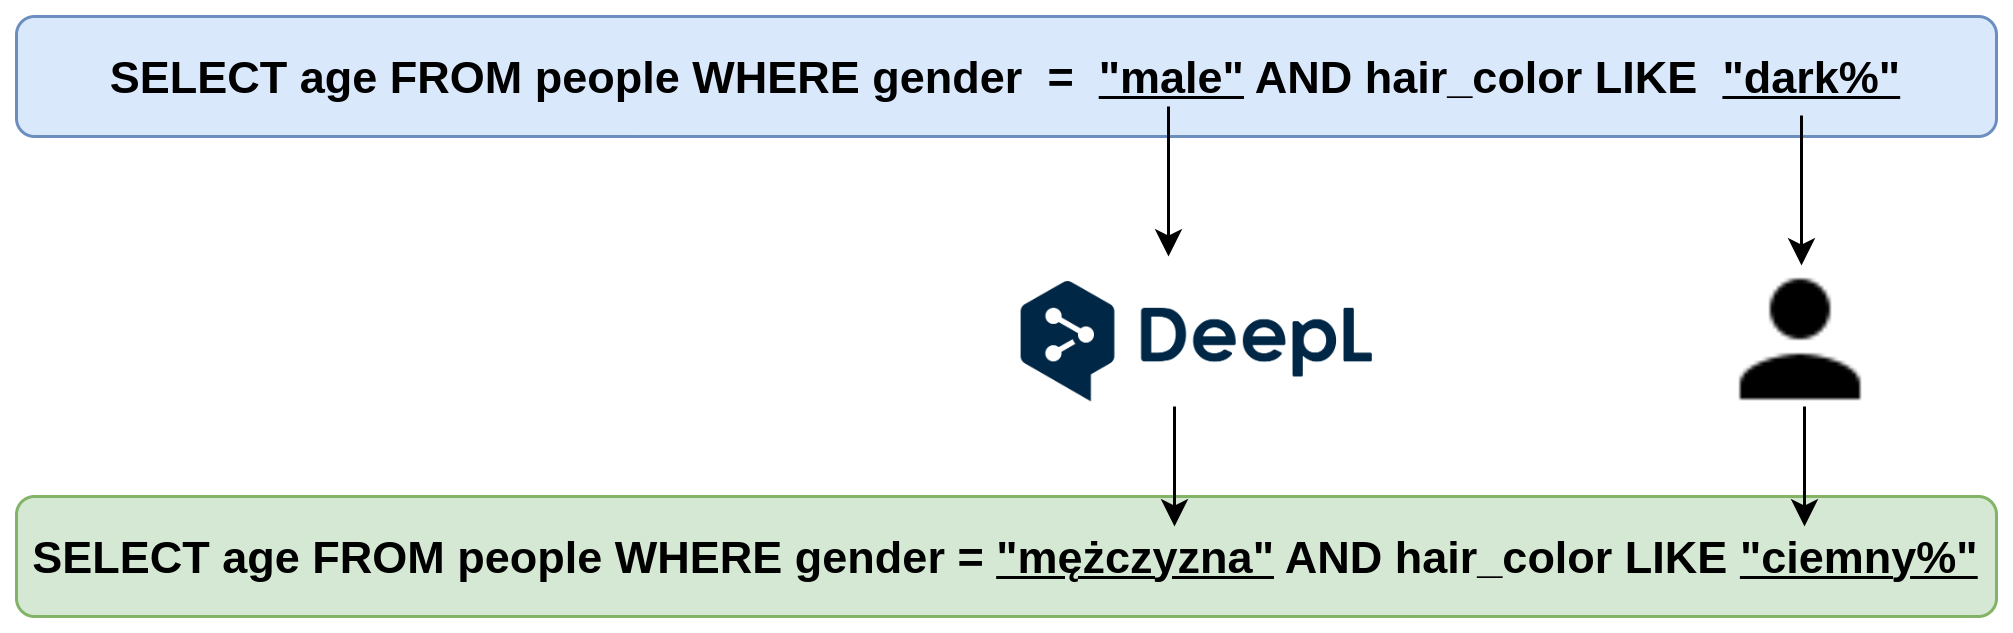
\includegraphics[width=1.0\linewidth]{images/value_translation.png}
  \caption{Wizualizacja etapu tłumaczenia wartości w zapytaniach SQL}
  \label{fig:value-translation}
\end{figure}

\section{Podsumowanie stworzonych zbiorów}
Niniejszy podrozdział stanowi ukoronowanie pracy nad polskimi zbiorami danych, ponieważ zawiera on przedstawienie i analizę przygotowanych zbiorów przykładów, tłumaczeń schematów oraz ostatecznie zbiorów, które poprzez ich kombinację można wygenerować.

\subsection{Przygotowane zbiory przykładów}

% \begin{table}[ht]
%     \centering
%     \begin{tabular}{|l|c|c|c|c|}
%         \hline
%         \thead{Zbiór} & 
%         \thead{Rodzaj\\tłumaczenia} &
%         \thead{Tłumaczenie\\schematu} &
%         \thead{Tłumaczenie\\zawartości\\baz danych} &
%         \thead{Tłumaczenie\\wartości w\\zapytaniach} \\
%         \hline
%         \makecell{Chiński\\(\code{CSpider})} & Manualne & Nie & Nie & Tak \\
%         \hline
%         \makecell{Wietnamski\\(\code{ViText2SQL})} & Manualne & Tak & Nie & Tak \\
%         \hline
%         \makecell{Portugalski} & Maszynowe & Tak & Nie & Nie \\
%         \hline
%         \makecell{Rosyjski\\(\code{PAUQ})} & Manualne & Nie & Częściowo & Tak \\
%         \hline
%     \end{tabular}
%     \caption{Zestawienie kluczowych różnic pomiędzy tłumaczeniami zbioru \code{Spider}}
%     \label{tab:spider-trans-diffs}
% \end{table}

\begin{table}[ht]
    \centering
    \begin{tabular}{|l|R{0.15\textwidth}|R{0.15\textwidth}|R{0.15\textwidth}|}
        \hline
        \thead{Zbiór} & \thead{Część\\treningowa} & \thead{Część\\walidacyjna} & \thead{Razem} \\
        \hline
        Spider & 8659 & 1034 & 9693 \\
        \hline
        Spider-DK & 0 & 535 & 535 \\
        \hline
        Spider-Syn & 3556 & 773 & 4329 \\
        \hline
        CoSQL & 1562 & 230 & 1792 \\
        \hline
        SParC & 2651 & 366 & 3017 \\
        \hhline{|=|=|=|=|} 
        Razem & 16428 & 2938 & 19366 \\
        \hline
    \end{tabular}
    \caption{Zestawienie liczby próbek w poszczególnych zbiorach}
    \label{tab:samples-count}
\end{table}

\begin{table}[ht]
    \centering
    \begin{tabular}{|l|R{0.15\textwidth}|R{0.15\textwidth}|R{0.15\textwidth}|R{0.15\textwidth}|R{0.15\textwidth}|}
        \hline
        \thead{Zbiór} & \thead{Easy} & \thead{Medium} & \thead{Hard} & \thead{Extra hard} \\
        \hline
        Spider & 2231 (23\%) & 3445 (36\%) & 2095 (22\%) & 1922 (20\%) \\
        \hline
        Spider-DK & 110 (21\%) & 246 (46\%) & 74 (14\%) & 105 (20\%) \\
        \hline
        Spider-Syn & 952 (22\%) & 1825 (42\%) & 884 (20\%) & 668 (15\%) \\
        \hline
        CoSQL & 949 (53\%) & 488 (27\%) & 222 (12\%) & 133 (\s7\%) \\
        \hline
        SParC & 2131 (71\%) & 706 (23\%) & 138 (\s5\%) & 42 (\s1\%) \\
        \hhline{|=|=|=|=|=|} 
        Wszystkie & 6373 (33\%) & 6710 (35\%) & 3413 (18\%) & 2870 (15\%) \\
        \hline
    \end{tabular}
    \caption{Zestawienia liczby próbek o poszczególnych poziomach trudności}
    \label{tab:difficulty}
\end{table}

% \begin{table}[ht]
%     \centering
%     \begin{tabular}{|l|R{0.15\textwidth}|R{0.15\textwidth}|R{0.15\textwidth}|}
%         \hline
%         \thead{Zbiór} & \thead{Min} & \thead{Max} & \thead{Średnia} \\
%         \hline
%         Spider & 3\s / \s3 & 224 / 227 & 66,74 / 66,44 \\
%         \hline
%         Spider-DK & 21 / 15 & 152 / 159 & 66,01 / 65,93 \\
%         \hline
%         Spider-Syn & 20 / 16 & 222 / 234 & 74,03 / 74,14 \\
%         \hline
%         CoSQL & 17 / 14 & 147 / 201 & 53,05 / 52,66 \\
%         \hline
%         SParC & 15 / 13 & 122 / 139 & 44,94 / 45,52 \\
%         \hhline{|=|=|=|=|} 
%         Wszystkie & 3\s / \s3 & 224 / 234 & 63,69 / 63,61 \\
%         \hline
%     \end{tabular}
%     \caption[Zestawienie liczby znaków polskich i angielskich pytań]{Zestawienie liczby znaków polskich i angielskich pytań (en / pl)}
%     \label{tab:questions-lengths}
% \end{table}

% \begin{table}[ht]
%     \centering
%     \begin{tabular}{|l|R{0.15\textwidth}|R{0.15\textwidth}|R{0.15\textwidth}|}
%         \hline
%         \thead{Zbiór} & \thead{Min} & \thead{Max} & \thead{Średnia} \\
%         \hline
%         Spider & 2 / 2 & 58 / 63 & 10,66 / 11,28 \\
%         \hline
%         Spider-DK & 3 / 3 & 28 / 28 & 8,47 / 8,59 \\
%         \hline
%         Spider-Syn & 2 / 2 & 39 / 54 & 9,65 / 10,28 \\
%         \hline
%         CoSQL & 3 / 3 & 51 / 66 & 10,11 / 10,72 \\
%         \hline
%         SParC & 3 / 3 & 45 / 55 & 10,24 / 10,84 \\
%         \hhline{|=|=|=|=|} 
%         Wszystkie & 2 / 2 & 58 / 66 & 10,32 / 10,94 \\
%         \hline
%     \end{tabular}
%     \caption[Zestawienie liczby znaków polskich i angielskich wartości z zapytań]{Zestawienie liczby znaków polskich i angielskich wartości z zapytań (en / pl)}
%     \label{tab:questions-lengths}
% \end{table}

\begin{table}[ht]
    \centering
    \begin{tabular}{|l|R{0.15\textwidth}|R{0.15\textwidth}|R{0.15\textwidth}|}
        \hline
        \thead{Zbiór} & \thead{Pytania} & \thead{Wartości} \\
        \hline
        Spider & 66,74 / 66,44 & 10,66 / 11,28 \\
        \hline
        Spider-DK & 66,01 / 65,93 & \s8,47 / \s8,59 \\
        \hline
        Spider-Syn & 74,03 / 74,14 & 9,65 / 10,28 \\
        \hline
        CoSQL & 53,05 / 52,66 & 10,11 / 10,72 \\
        \hline
        SParC & 44,94 / 45,52 & 10,24 / 10,84 \\
        \hhline{|=|=|=|} 
        Wszystkie & 63.69 / 63.61 & 10,32 / 10,94 \\
        \hline
    \end{tabular}
    \caption[Zestawienie liczby znaków w pytaniach i wartościach dla języka angielskiego i polskiego]{Zestawienie liczby znaków w pytaniach i wartościach dla języka angielskiego i polskiego (en / pl)}
    \label{tab:questions-lengths}
\end{table}

\subsection{Przygotowane tłumaczenia schematów}


\subsection{Nazwane warianty}

% Przedstawienie stworzonych zbiorów nie jest proste, ponieważ założeniem było, aby dla każdej wersji angielskiej nie powstało tylko jedno statyczne tłumaczenie, lecz aby można było wygenerować różne polskie warianty. Nie mniej jednak w celu ułatwienia dalszej pracy poprzez możliwość odwoływania się do konkretnych zbiorów to kilka wariantów zostało zdefiniowanych i nazwanych. Ponadto zdefiniowane i nazwane zostały również pewne połączenia tych zbiorów, do których występują częste odwołania. 

W celu ułatwienia dalszej pracy poprzez możliwość odwoływania się do konkretnych zbiorów kilka wariantów zbiorów zostało nazwanych. Ponadto zdefiniowane zostały również pewne połączenia tych zbiorów, ponieważ występują do nich częste odwołania.

\begin{figure}[ht!]
  \centering
  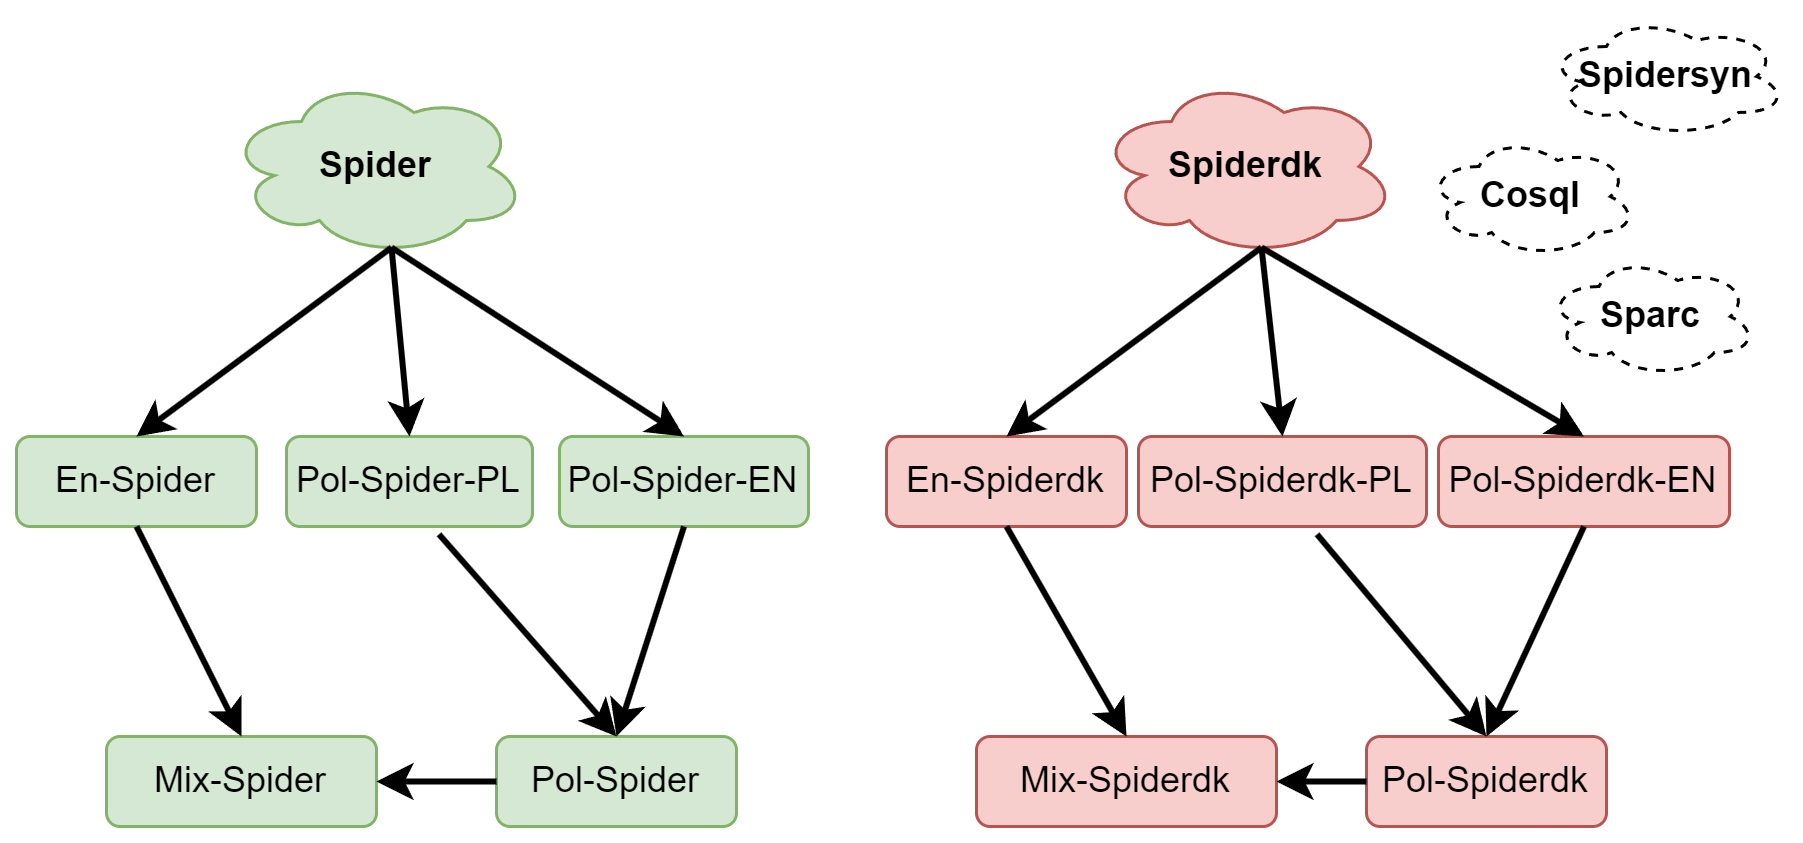
\includegraphics[width=1.0\linewidth]{images/datasets.png}
  \caption{Schemat zależności pomiędzy zbudowanymi zbiorami danych}
  \label{fig:datasets}
\end{figure}

Schemat zdefiniowanych zbiorów został przedstawiony na rysunku \ref{fig:datasets}. Można z niego odczytać, że na bazie zbioru \code{Spider} wygenerowane zostały trzy warianty. \code{En-Spider} to wariant całkowicie angielski, bardzo podobny do oryginalnego \code{Spider}, ale z minimalnymi różnicami, jak sposób tokenizacji. \code{Pol-Spider-PL} to wariant polski z polskim schematem baz danych, a \code{Pol-Spider-EN} to wariant polski z angielskim schematem baz danych. Te dwa polskie warianty zostały połączone w zbiór \code{Pol-Spider}, który jest więc polskim zbiorem zawierającym schematy baz danych w obu popularnych wariantach. Ponadto często wykorzystywane jest złączenie zbioru przetłumaczonego z angielskim więc połączenie zbioru \code{Pol-Spider} oraz \code{En-Spider} nazwano \code{Mix-Spider}. Podobny schemat nazewnictwa został zastosowany do reszty zbiorów. Schematyczne i wymowne nazwy powinny ułatwić zapamiętanie tych relacji.

% Ponadto stworzone i nazwane zostały globalne złączenia pomiędzy wszystkimi opisanymi powyżej wariantami. \code{Ultimate} zawiera wszystkie całkowicie angielskie warianty. \code{Pol-Ultimate-EN} oraz \code{Pol-Ultimate-PL} zawierają wszystkie polskie warianty z odpowiednio angielskimi i polskimi schematami baz danych. \code{Pol-Ultimate} agreguje dwa powyższe, a \code{Pol-Ultimate-Mix} dodatkowo dodaje do tego warianty angielskie. 


Należy zaznaczyć, że warianty zawierające schemat baz danych w języku polskim nie zawierają tam polskich znaków. Bezproblemowe byłoby wygenerowanie również zbiorów, które zawierałyby polskie znaki w schemacie, lecz jest to tak rzadko spotykany w praktyce przypadek, że nie był brany pod uwagę.

